\subsection{Description du projet}
La societe Infineon Technologie GA propone un gateway securis\'e KIT\_A2G\_TC377\_SEC\_GTW \cite{gateway} (fig \ref{fig:gw-photo}) el cual corre con un microcontrolador \textit{AURIX TC37xEXT} para poder aumentar la conectividad de diferentes redes como el FlexRay, LIN, CAN y Ethernet dentro del automobil. El sistema operativo usado dentro de este gateway es fourni por Vector Informatik y se llama MICROSAR Classic \cite{vector.microsar}. Este sistema operativo es totalmente compatible con AUTOSAR lo cual nos deja con una ECU 100\% funcional sobre la cual se pueden correr software components (swc) compatibles con AUTOSAR. Ademas tambien se utilisa un switch ethernet securis\'e Marvell 88Q5050 que permite velocidad y ancho de banda estables con toda la seguridad que un automobil requiere.

\begin{figure}[!htb]
 \centering
 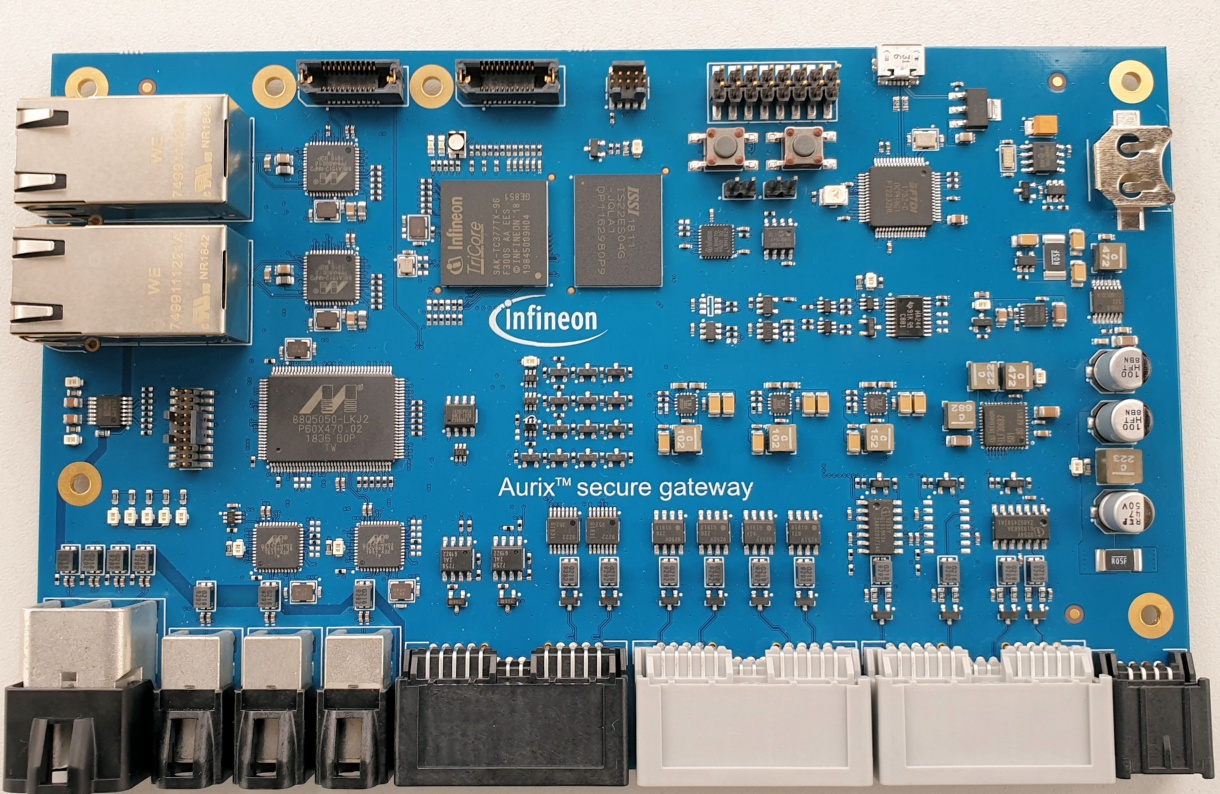
\includegraphics[width=0.8\textwidth]{img/secure-gateway.jpg}
 \caption{KIT\_A2G\_TC377\_SEC\_GTW}
 \label{fig:gw-photo}
\end{figure}

El gateway viene con un programa de demostracion que pretende hacer la prise en main del gateway, testear el funcionamiento basico y mostrar las capacidades del mismo. Para testear el Demo es necesario conectar 2 ECU's externar a ciertos puertos especificados en la figura \ref{fig:connections-diagram}. El demo en cuestion tiene 2 use Cases los cuales vamos a explicar por separado.

\begin{itemize}
    \item Use Case 1 : En este Use Case se envia un frame can y el gateway le hace forward por puerto ethernet. Retratado en la figura \ref{fig:gw-demo-uc1}.
    \item Use Case 2 : En Este Use case se envia un frame ethernet y esto se le hace forward hacia un bus can. Retratado en la figura \ref{fig:gw-demo-uc2}.
\end{itemize}

\begin{figure}[!htb]
 \centering
 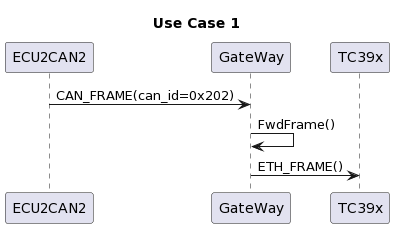
\includegraphics[width=0.5\textwidth]{img/GWUseCase1.png}
 \caption{Gateway Demo Use Case 1}
 \label{fig:gw-demo-uc1}
\end{figure}

\begin{figure}[!htb]
 \centering
 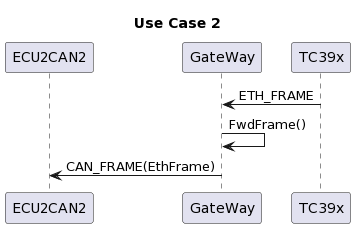
\includegraphics[width=0.5\textwidth]{img/GWUseCase2.png}
 \caption{Gateway Demo Use Case 2}
 \label{fig:gw-demo-uc2}
\end{figure}

\subsection{Objectifs du projet}

La propuesta de ASTC Desing Partners es virtualizar este Gateway para poder agilizar el proceso del desarrollo de software, sobretodo en un contexto de escasez mundial de microcontroladores. Ademas, es bien sabido que suele haber pocas unidades disponibles para testear por lo que es mejor tenerlo digitalizado para que cada programador pueda avanzar por su lado sin necesidad de hacer cola por el hardware, a menos que sea necesario.

Bien si vlab puede correr el microcontrolador, este gateway tiene otros componentes con los que se interactua y por tanto puede suponer un problema si no estan presentes asi que otro de los objetivos es modelizar circuitos y buses de datos que esten conectados entre si para que el software pueda arrancar.
\begin{itemize}
    \item Modelar componentes necesarios para hacer arrancar el gateway
    \item Hacer un testbench con los componentes necesarios conectados
    \item Configurar Vlab para que corra MICROSAR Classic
\end{itemize}